\documentclass[twoside]{book}

% Packages required by doxygen
\usepackage{fixltx2e}
\usepackage{calc}
\usepackage{doxygen}
\usepackage[export]{adjustbox} % also loads graphicx
\usepackage{graphicx}
\usepackage[utf8]{inputenc}
\usepackage{makeidx}
\usepackage{multicol}
\usepackage{multirow}
\PassOptionsToPackage{warn}{textcomp}
\usepackage{textcomp}
\usepackage[nointegrals]{wasysym}
\usepackage[table]{xcolor}

% Font selection
\usepackage[T1]{fontenc}
\usepackage[scaled=.90]{helvet}
\usepackage{courier}
\usepackage{amssymb}
\usepackage{sectsty}
\renewcommand{\familydefault}{\sfdefault}
\allsectionsfont{%
  \fontseries{bc}\selectfont%
  \color{darkgray}%
}
\renewcommand{\DoxyLabelFont}{%
  \fontseries{bc}\selectfont%
  \color{darkgray}%
}
\newcommand{\+}{\discretionary{\mbox{\scriptsize$\hookleftarrow$}}{}{}}

% Page & text layout
\usepackage{geometry}
\geometry{%
  a4paper,%
  top=2.5cm,%
  bottom=2.5cm,%
  left=2.5cm,%
  right=2.5cm%
}
\tolerance=750
\hfuzz=15pt
\hbadness=750
\setlength{\emergencystretch}{15pt}
\setlength{\parindent}{0cm}
\setlength{\parskip}{3ex plus 2ex minus 2ex}
\makeatletter
\renewcommand{\paragraph}{%
  \@startsection{paragraph}{4}{0ex}{-1.0ex}{1.0ex}{%
    \normalfont\normalsize\bfseries\SS@parafont%
  }%
}
\renewcommand{\subparagraph}{%
  \@startsection{subparagraph}{5}{0ex}{-1.0ex}{1.0ex}{%
    \normalfont\normalsize\bfseries\SS@subparafont%
  }%
}
\makeatother

% Headers & footers
\usepackage{fancyhdr}
\pagestyle{fancyplain}
\fancyhead[LE]{\fancyplain{}{\bfseries\thepage}}
\fancyhead[CE]{\fancyplain{}{}}
\fancyhead[RE]{\fancyplain{}{\bfseries\leftmark}}
\fancyhead[LO]{\fancyplain{}{\bfseries\rightmark}}
\fancyhead[CO]{\fancyplain{}{}}
\fancyhead[RO]{\fancyplain{}{\bfseries\thepage}}
\fancyfoot[LE]{\fancyplain{}{}}
\fancyfoot[CE]{\fancyplain{}{}}
\fancyfoot[RE]{\fancyplain{}{\bfseries\scriptsize Generated by Doxygen }}
\fancyfoot[LO]{\fancyplain{}{\bfseries\scriptsize Generated by Doxygen }}
\fancyfoot[CO]{\fancyplain{}{}}
\fancyfoot[RO]{\fancyplain{}{}}
\renewcommand{\footrulewidth}{0.4pt}
\renewcommand{\chaptermark}[1]{%
  \markboth{#1}{}%
}
\renewcommand{\sectionmark}[1]{%
  \markright{\thesection\ #1}%
}

% Indices & bibliography
\usepackage{natbib}
\usepackage[titles]{tocloft}
\setcounter{tocdepth}{3}
\setcounter{secnumdepth}{5}
\makeindex

% Hyperlinks (required, but should be loaded last)
\usepackage{ifpdf}
\ifpdf
  \usepackage[pdftex,pagebackref=true]{hyperref}
\else
  \usepackage[ps2pdf,pagebackref=true]{hyperref}
\fi
\hypersetup{%
  colorlinks=true,%
  linkcolor=blue,%
  citecolor=blue,%
  unicode%
}

% Custom commands
\newcommand{\clearemptydoublepage}{%
  \newpage{\pagestyle{empty}\cleardoublepage}%
}

\usepackage{caption}
\captionsetup{labelsep=space,justification=centering,font={bf},singlelinecheck=off,skip=4pt,position=top}

%===== C O N T E N T S =====

\begin{document}

% Titlepage & ToC
\hypersetup{pageanchor=false,
             bookmarksnumbered=true,
             pdfencoding=unicode
            }
\pagenumbering{roman}
\begin{titlepage}
\vspace*{7cm}
\begin{center}%
{\Large My Project }\\
\vspace*{1cm}
{\large Generated by Doxygen 1.8.11}\\
\end{center}
\end{titlepage}
\clearemptydoublepage
\tableofcontents
\clearemptydoublepage
\pagenumbering{arabic}
\hypersetup{pageanchor=true}

%--- Begin generated contents ---
\chapter{Hierarchical Index}
\section{Class Hierarchy}
This inheritance list is sorted roughly, but not completely, alphabetically\+:\begin{DoxyCompactList}
\item \contentsline{section}{Console\+For\+Timetable}{\pageref{class_console_for_timetable}}{}
\item \contentsline{section}{Core\+\_\+of\+\_\+timetable}{\pageref{class_core__of__timetable}}{}
\item exception\begin{DoxyCompactList}
\item \contentsline{section}{Insufficient\+Rights}{\pageref{class_insufficient_rights}}{}
\end{DoxyCompactList}
\item Q\+Main\+Window\begin{DoxyCompactList}
\item \contentsline{section}{Main\+Window}{\pageref{class_main_window}}{}
\end{DoxyCompactList}
\end{DoxyCompactList}

\chapter{Class Index}
\section{Class List}
Here are the classes, structs, unions and interfaces with brief descriptions\+:\begin{DoxyCompactList}
\item\contentsline{section}{\hyperlink{class_beyond_the_array}{Beyond\+The\+Array} \\*Выход за пределы массива }{\pageref{class_beyond_the_array}}{}
\item\contentsline{section}{\hyperlink{class_console_for_timetable}{Console\+For\+Timetable} \\*Класс служащий для работы с ядром через консоль }{\pageref{class_console_for_timetable}}{}
\item\contentsline{section}{\hyperlink{class_core_of_timetable}{Core\+Of\+Timetable} \\*Класс в котором содержится бизнес-\/логика приложения }{\pageref{class_core_of_timetable}}{}
\item\contentsline{section}{\hyperlink{class_failed_to_open}{Failed\+To\+Open} \\*Не удалось открыть файл }{\pageref{class_failed_to_open}}{}
\item\contentsline{section}{\hyperlink{class_file_timetable}{File\+Timetable} \\*Смысл класса в обмене информации между ядром и файлом }{\pageref{class_file_timetable}}{}
\item\contentsline{section}{\hyperlink{class_main_window}{Main\+Window} \\*Класс служащий для работы с \char`\"{}\+Core\+\_\+of\+\_\+timetable\char`\"{} через графическую оболочку(будет реализован не скоро) }{\pageref{class_main_window}}{}
\item\contentsline{section}{\hyperlink{class_test__for__core_test}{Test\+\_\+for\+\_\+core\+Test} \\*Тесты для ядра }{\pageref{class_test__for__core_test}}{}
\end{DoxyCompactList}

\chapter{Class Documentation}
\hypertarget{class_console_for_timetable}{}\section{Console\+For\+Timetable Class Reference}
\label{class_console_for_timetable}\index{Console\+For\+Timetable@{Console\+For\+Timetable}}


{\ttfamily \#include $<$console\+\_\+for\+\_\+timetable.\+h$>$}



\subsection{Detailed Description}
Класс служащий для работы с ядром через консоль 

The documentation for this class was generated from the following files\+:\begin{DoxyCompactItemize}
\item 
Console\+\_\+for\+\_\+timetable/console\+\_\+for\+\_\+timetable.\+h\item 
Console\+\_\+for\+\_\+timetable/console\+\_\+for\+\_\+timetable.\+cpp\end{DoxyCompactItemize}

\hypertarget{class_core__of__timetable}{}\section{Core\+\_\+of\+\_\+timetable Class Reference}
\label{class_core__of__timetable}\index{Core\+\_\+of\+\_\+timetable@{Core\+\_\+of\+\_\+timetable}}


{\ttfamily \#include $<$core\+\_\+of\+\_\+timetable.\+h$>$}

\subsection*{Public Member Functions}
\begin{DoxyCompactItemize}
\item 
void {\bfseries issuance\+Of\+Administrator\+Rights} ()\hypertarget{class_core__of__timetable_a9ec4d33c0d66d515f22e56653a2c77ea}{}\label{class_core__of__timetable_a9ec4d33c0d66d515f22e56653a2c77ea}

\item 
int {\bfseries information\+Of\+The\+Rights} ()\hypertarget{class_core__of__timetable_a51ce39ebdcd1d1e072cd06f145aa94a0}{}\label{class_core__of__timetable_a51ce39ebdcd1d1e072cd06f145aa94a0}

\item 
vector$<$ string $>$ $\ast$ {\bfseries timetable\+For\+Train} (int number\+\_\+of\+\_\+the\+\_\+train)\hypertarget{class_core__of__timetable_aa96d8324770692f0aa814d3c8210fc4a}{}\label{class_core__of__timetable_aa96d8324770692f0aa814d3c8210fc4a}

\end{DoxyCompactItemize}


\subsection{Detailed Description}
Класс в котором содержится бизнес-\/логика приложения 

The documentation for this class was generated from the following files\+:\begin{DoxyCompactItemize}
\item 
Core\+\_\+of\+\_\+timetable/core\+\_\+of\+\_\+timetable.\+h\item 
Core\+\_\+of\+\_\+timetable/core\+\_\+of\+\_\+timetable.\+cpp\end{DoxyCompactItemize}

\hypertarget{class_insufficient_rights}{}\section{Insufficient\+Rights Class Reference}
\label{class_insufficient_rights}\index{Insufficient\+Rights@{Insufficient\+Rights}}
Inheritance diagram for Insufficient\+Rights\+:\begin{figure}[H]
\begin{center}
\leavevmode
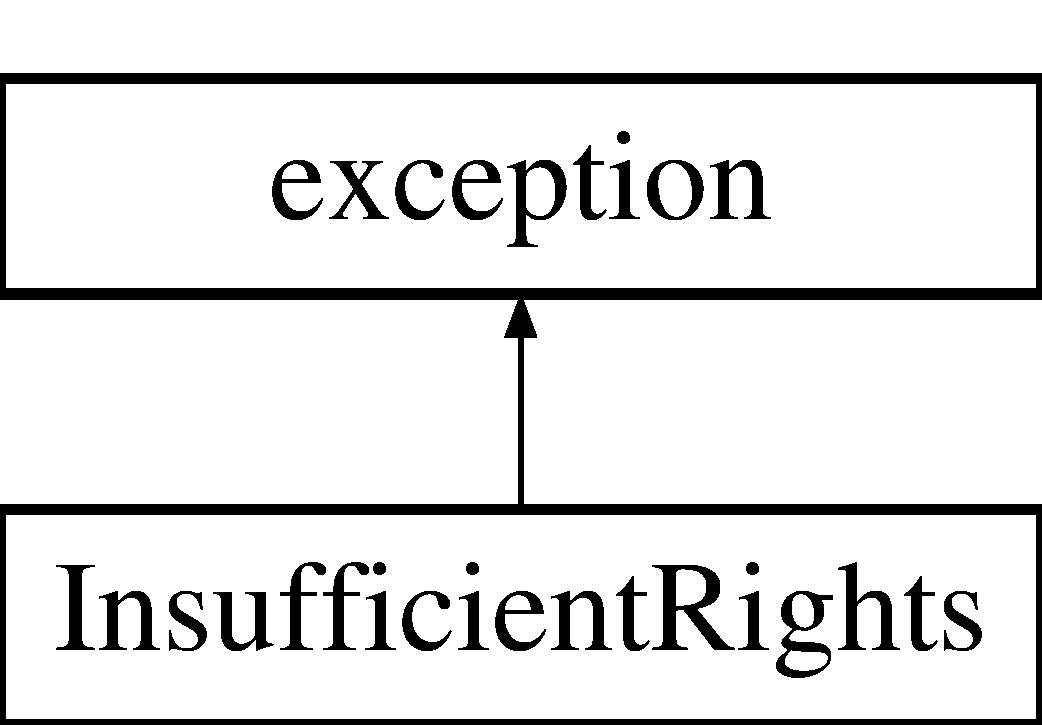
\includegraphics[height=2.000000cm]{class_insufficient_rights}
\end{center}
\end{figure}


The documentation for this class was generated from the following file\+:\begin{DoxyCompactItemize}
\item 
Console\+\_\+for\+\_\+timetable/console\+\_\+for\+\_\+timetable.\+h\end{DoxyCompactItemize}

\hypertarget{class_main_window}{}\section{Main\+Window Class Reference}
\label{class_main_window}\index{Main\+Window@{Main\+Window}}


Класс служащий для работы с \char`\"{}\+Core\+\_\+of\+\_\+timetable\char`\"{} через графическую оболочку(будет реализован не скоро)  




{\ttfamily \#include $<$mainwindow.\+h$>$}

Inheritance diagram for Main\+Window\+:\begin{figure}[H]
\begin{center}
\leavevmode
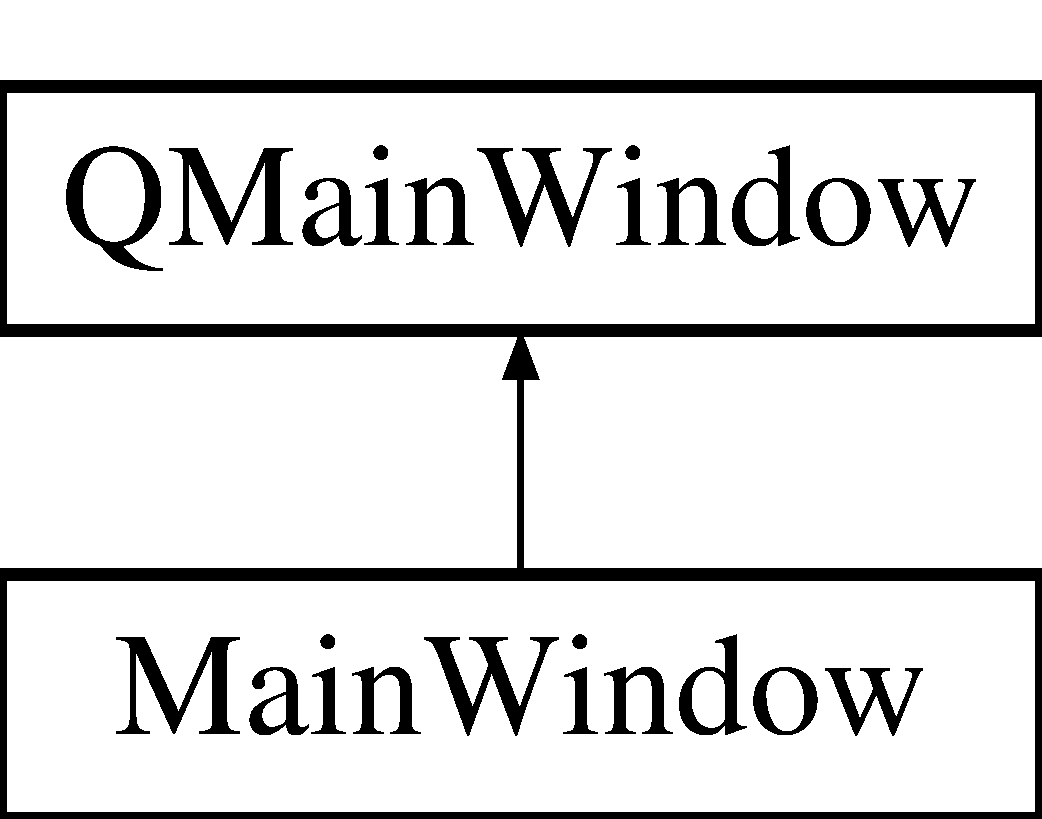
\includegraphics[height=2.000000cm]{class_main_window}
\end{center}
\end{figure}
\subsection*{Public Member Functions}
\begin{DoxyCompactItemize}
\item 
{\bfseries Main\+Window} (Q\+Widget $\ast$parent=0)\hypertarget{class_main_window_a8b244be8b7b7db1b08de2a2acb9409db}{}\label{class_main_window_a8b244be8b7b7db1b08de2a2acb9409db}

\end{DoxyCompactItemize}


\subsection{Detailed Description}
Класс служащий для работы с \char`\"{}\+Core\+\_\+of\+\_\+timetable\char`\"{} через графическую оболочку(будет реализован не скоро) 

The documentation for this class was generated from the following files\+:\begin{DoxyCompactItemize}
\item 
G\+U\+I\+\_\+for\+\_\+timetable/mainwindow.\+h\item 
G\+U\+I\+\_\+for\+\_\+timetable/mainwindow.\+cpp\end{DoxyCompactItemize}

%--- End generated contents ---

% Index
\backmatter
\newpage
\phantomsection
\clearemptydoublepage
\addcontentsline{toc}{chapter}{Index}
\printindex

\end{document}
